\documentclass{sigchi}

% Use this command to override the default ACM copyright statement
% (e.g. for preprints).  Consult the conference website for the
% camera-ready copyright statement.

%% EXAMPLE BEGIN -- HOW TO OVERRIDE THE DEFAULT COPYRIGHT STRIP -- (July 22, 2013 - Paul Baumann)
% \toappear{Permission to make digital or hard copies of all or part of this work for personal or classroom use is      granted without fee provided that copies are not made or distributed for profit or commercial advantage and that copies bear this notice and the full citation on the first page. Copyrights for components of this work owned by others than ACM must be honored. Abstracting with credit is permitted. To copy otherwise, or republish, to post on servers or to redistribute to lists, requires prior specific permission and/or a fee. Request permissions from permissions@acm.org. \\
% {\emph{CHI'14}}, April 26--May 1, 2014, Toronto, Canada. \\
% Copyright \copyright~2014 ACM ISBN/14/04...\$15.00. \\
% DOI string from ACM form confirmation}
%% EXAMPLE END -- HOW TO OVERRIDE THE DEFAULT COPYRIGHT STRIP -- (July 22, 2013 - Paul Baumann)

% Arabic page numbers for submission.  Remove this line to eliminate
% page numbers for the camera ready copy
% \pagenumbering{arabic}

% Load basic packages
\usepackage{balance}  % to better equalize the last page
\usepackage{graphics} % for EPS, load graphicx instead 
\usepackage[T1]{fontenc}
\usepackage{txfonts}
\usepackage{mathptmx}
\usepackage[pdftex]{hyperref}
\usepackage{color}
\usepackage{booktabs}
\usepackage{textcomp}
% Some optional stuff you might like/need.
\usepackage{microtype} % Improved Tracking and Kerning
% \usepackage{hypercap}  % Fixes bug in hyperref caption linking
\usepackage{ccicons}  % Cite your images correctly!
% \usepackage[utf8]{inputenc} % for a UTF8 editor only

% If you want to use todo notes, marginpars etc. during creation of your draft document, you
% have to enable the "chi_draft" option for the document class. To do this, change the very first
% line to: "\documentclass[chi_draft]{sigchi}". You can then place todo notes by using the "\todo{...}"
% command. Make sure to disable the draft option again before submitting your final document.
\usepackage{todonotes}

% Paper metadata (use plain text, for PDF inclusion and later
% re-using, if desired).  Use \emtpyauthor when submitting for review
% so you remain anonymous.
\def\plaintitle{Lightweight Document Classification for Device-based APP-Recommendation: A Graph-based Approach}
\def\plainauthor{% ANONYMISEDFirst Author, Second Author, Third Author,
}
\def\emptyauthor{}
\def\plainkeywords{App recommendation; Document classification; Summarization}
\def\plaingeneralterms{Document classification}

% llt: Define a global style for URLs, rather that the default one
\makeatletter
\def\url@leostyle{%
  \@ifundefined{selectfont}{
    \def\UrlFont{\sf}
  }{
    \def\UrlFont{\small\bf\ttfamily}
  }}
\makeatother
\urlstyle{leo}

% To make various LaTeX processors do the right thing with page size.
\def\pprw{8.5in}
\def\pprh{11in}
\special{papersize=\pprw,\pprh}
\setlength{\paperwidth}{\pprw}
\setlength{\paperheight}{\pprh}
\setlength{\pdfpagewidth}{\pprw}
\setlength{\pdfpageheight}{\pprh}

% Make sure hyperref comes last of your loaded packages, to give it a
% fighting chance of not being over-written, since its job is to
% redefine many LaTeX commands.
\definecolor{linkColor}{RGB}{6,125,233}
\hypersetup{%
  pdftitle={\plaintitle},
% Use \plainauthor for final version.
%  pdfauthor={\plainauthor},
  pdfauthor={\emptyauthor},
  pdfkeywords={\plainkeywords},
  bookmarksnumbered,
  pdfstartview={FitH},
  colorlinks,
  citecolor=black,
  filecolor=black,
  linkcolor=black,
  urlcolor=linkColor,
  breaklinks=true,
}

% create a shortcut to typeset table headings
% \newcommand\tabhead[1]{\small\textbf{#1}}

% End of preamble. Here it comes the document.
\begin{document}

\title{\plaintitle}

\numberofauthors{3}
\author{%
% ANONYMISED
%   \alignauthor{1st Author Name\\
%     \affaddr{Affiliation}\\
%     \affaddr{City, Country}\\
%     \email{e-mail address}}\\
%   \alignauthor{2nd Author Name\\
%     \affaddr{Affiliation}\\
%     \affaddr{City, Country}\\
%     \email{e-mail address}}\\
%   \alignauthor{3rd Author Name\\
%     \affaddr{Affiliation}\\
%     \affaddr{City, Country}\\
%     \email{e-mail address}}\\
}

\maketitle

\begin{abstract}
We consider the problem of lift document classification on mobile devices.
Document classification is the task of automatically assigning a set of unlabeled documents into a set of predefined categories.
This technique is relevant for app-recommendation systems on mobile phones. 
While app-stores provide basic recommendation functionality, more advanced recommendation systems require fine-grained usage information available only locally on the mobile device. 
However, due to severe resource restrictions on such devices, computational cost needs to be optimised. 
In this paper, summarization as an approach to circumvent the curse of dimensionality is investigated. 
High dimensional feature space can be reduced significantly by considering summarized document as a feature set, since it includes the most important information of the original document. 
Graph-based summarization technique is applied on the classification process, and remarkably improves the performance of document classification.
\end{abstract}

\category{H.5.m.}{Information Interfaces and Presentation
  (e.g. HCI)}{Miscellaneous} \category{See
  \url{http://acm.org/about/class/1998/} for the full list of ACM
  classifiers. This section is required.}{}{}

\keywords{\plainkeywords}

\section{Introduction}
It has become easy to find an app for virtually any possible category but challenging to identify good and reliable apps from this overwhelming choice. 
Although app-stores typically provide basic recommendation functionality, such systems favor apps with a bigger crowd of users such as corporation-developed apps or older and therefore better known apps.
They can not take into account the individual interest of users and their usage habits. 
This problem has been tackled by app recommendation systems which require local installation~\cite{Yan-mobisys-2011,Shi-sigkdd-2012}.
However, these systems are highly resource demanding and therefore not applicable in practical everyday use.
What is required is a computationally cheap approach that is feasible for the application on end-user mobile devices. 
In this paper, we tackle this problem by considering summarization as an approach to circumvent the curse of dimensionality in document classification.

Automatic document classification (also known as text categorization, or topic spotting) is the task of automatically sorting a set of documents into categories (or classes, or topics) from a predefined set~\cite{Sebastiani:2002:MLA:505282.505283}. 
For app-recommendation systems, document classification is an essential component to group apps into categories according to their textual description, crawled, for instance, from online-appstores. 

In document classification, one document is often represented as a vector of words (bag of words), and all these words are not that informative to be included in the final feature set. 
Therefore feature selection should be applied not only to select the most relevant features, but to reduce the high dimensionality of feature vector space. 
In this paper, text summarization will be considered as a feature selection technique to extract the least number of features with the most informativeness for each category.

Online app-stores and the description of apps therein are subject to constant change. 
Furthermore, a ground truth for correct classification is naturally missing. 
In order to produce comparable results and to reliably measure the performance of our approach, we apply our approach to the Reuters-21578 corpus which is a standard benchmark for document classification. 
It has been employed in multiple scientific publications in many research areas especially in information retrieval, natural language
processing and machine learning. 
The hidden semantic relationship between some categories and the skewed distribution of documents make Reuters-21578 corpus most
interesting for document classification with respect to app recommendation systems~\cite{debole2005analysis}. 
Moreover, it has several categories which own very few positive training examples; challenging the performance of the document classification system based on machine learning methods.
The documents refer to the Reuters newswire in 1987 and the classification was done manually by personnel from Reuters Ltd. 
Due to its large number of categories, different subsets of its categories have been adopted as dataset. 
A subset of~30 categories will be taken into account for this project, with at least one positive training example and one test example.

The rest of this document is orgainzed as follows. 
In Section~\ref{sectionRelatedWork}, related work is reviewed. 
Section~\ref{sectionMethodology} presents our approach.
Section~\ref{sectionExperiments} details our results and section~\ref{sectionConclusion} concludes the discussion.

\section{Related Work}\label{sectionRelatedWork}
Application recommenders have started to become increasingly commonplace, with several academic~\cite{Yan-mobisys-2011,Shi-sigkdd-2012} and commercial systems~\footnote{The Aptoide meta-store: \url{http://m.aptoide.com/}} %% I did not find any. Do we have examples for these?
emerging in recent years. 
Some of these operate as separate applications that are installed on the device, such as Aptoide and Cydia, but some, like Aptoide, can also be reached through a web browser on another device.
%TODO: Actually, I think this is illegal. There's a store in China that swipes apps from Google Play. with the marketplace itself~\cite{?}. %%Here again: Could not find an app to search apps. 
At the same time, recommendations have started to emerge on the marketplaces themselves, e.g. Google Play supports both personalized recommendations and country-specific "featured" and most popular application listings.

First works on mobile app recommendations were focused on adopting standard content-based and collaborative filtering techniques for generating recommendations. 
Most of these works operated directly on the marketplace and relied on application popularity, such as installation counts and click stream data, or ratings to generate recommendations~\cite{Bostrom:2008:CIU:1409240.1409280}. 
However, as shown by Falaki et al.~\cite{Falaki-mobisys-2010}, installation counts are a poor indicator of user interest as users tend to try out applications without necessarily ever using them again.
The same holds for ratings which do not necessarily reflect true user interest~\cite{Yan-mobisys-2011}. 
At the same time, user habits and personalised usage patterns have a high potential to significantly improve app recommendation systems~\cite{Bohmer-mobilechi-2011}.

Motivated by these findings, most recent work on app recommendation relies on usage information gathered directly from the device. 
For example, AppJoy~\cite{Yan-mobisys-2011} considers a weighted model where recency, frequency, and duration of interactions are taken into consideration, whereas GetJar~\cite{Shi-sigkdd-2012} and the Djinn system of Karatzoglou et al.~\cite{Karatzoglou-cikm-2012} consider information derived from binary usage patterns. AppJoy relies on a constantly running background process that monitors app use, while both GetJar and our technique can be used with crowdsourced,
infrequently sampled data.
Both AppJoy and GetJar are based on standard recommender system techniques, whereas Djinn is based on tensor-factorization model that additionally considers also the usage context of applications. 
Also other works on integrating context information as part of app recommendations have been proposed~\cite{Mizzaro-carr-2014, Davidsson-carr-2011, woerndl-2007}. 

Recently, the AppTrends approach proposed to consider actual usage data and to base the recommendation on frequency of co-usage of apps~\cite{7072833}.
They show that recommendations should consider co-usage of apps as particular use cases on mobile devices involve a common set of apps rather than individual apps only. 
While these systems can provide better and more personalised recommendation results than the basic approaches provided via app stores, the high resource demands of the mobile-based solutions render practical use impossible.
We therefore investigate lightweight document classification to mitigate this problem.

Feature selection as a fundamental task plays an important role in the overall performance of automatic document classification. 
Many techniques and approaches has been studied and deployed in feature selection, which all focus on aggressive dimensionality reduction. 
Apart from common feature selection methods such as Document Frequency (DF), Information Gain (IG), Statistic and Mutual Information (MI), in several researches text summarization was applied as feature selection and it was found useful and beneficial in automatic document classification.

Ker and Chen~\cite{Ker:2000:TCB:1117755.1117766} proposed a summarization-based document classification system. 
Among Several techniques for text summarization (which includes methods based on position, cue phrase, word frequency and discourse segmentation) word-based frequency and position methods were considered and then combined to extract features. 
From position point of view, title of the document was only used with the assumption that existing words in the title likely describe the context relatively well.
After weighting the selected features, document classification was performed by a probabilistic classifier exploring TF-IDF (Term frequency–Inverse Document Frequency). 
The experiment showed that using title as a summarization technique would result in acceptable performance, meanwhile decline the execution time.

The work by Kolcz et al.~\cite{Kolcz:2001:SFS:502585.502647} tried to prove the efficiency of their proposed summarization technique by using it as a feature selection method in document classification. 
Different summarization methods based on the title of the story, paragraphs and best sentence were considered in the approach in order to reduce the feature set to a manageable size. Paragraphs' position, keywords and title words were taken into account in summary generation, which included first paragraph, first two paragraph, first last paragraph, paragraph with most keywords and paragraph with most title words. In addition, another summary was also constructed by choosing the sentences with at least 3 title words and at least 4 keywords. 
The applied classifier was a Support Vector Machine (SVM). 
The applied summarization methods were as effective as state-of-art statistical feature selection methods in DC, specially the best sentence-based summary.
In another text summarization method, Ko et al.~\cite{Ko:2004:ITC:975966.975971} determined the importance of sentences in a document by combining two methods. 
First, instead of directly using terms of the title, the most similar sentences with the title were selected, and then in the second method the sentence with the highest sum of weighted terms (based on TF, IDF, and X2 statistics values). 
Afterwards, the chosen sentences were scored by a modified weighting technique, to retrieve the most informative sentence. 
The suggested system enhanced the performance of document classification in four applied classifiers: Naive Bayes, Rocchio, k-NN, and SVM classifier, regardless of specific language.

Mihalcea and Hassan~\cite{mihalcea2005using} presented a new approach by summarizing the documents in order to improve and enhance the classifier which results in efficient execution of a document classification.
The extraction of sentences was performed with the aid of graph-based algorithms which ranked them according to the number of links. 
Two popular ranking algorithms, PageRank~\cite{Brin20123825} and HITS (Hyperlinked Induced Topic Search)~\cite{Kleinberg:1999:ASH:324133.324140} were deployed in order to decide on the importance of sentences which finally construct the summarization. 
Mapping these algorithms to the document, each sentence is considered as a vertice, and if each pair of sentences have some informative terms in common, then there will be an edge between them. 
Naive Bayes, Rocchio were applied as main classifiers. 
The results revealed that the proposed system improved the classification efficiency, disconsidering the length of the original document. 
The technique was also recommended as a measurement for different summarization tool evaluation.

Jiang et al.~\cite{4797414} examined the impact of summarzation on document classification, by considering two different applications of summary in order to obtain the feature set: the summary itself as the feature set and applying classical feature selection methods (MI, IG and DF) on the summary. 
To construct the summary, only nouns and verbs were weighted, with regard to semantic-based distance value and connective strength value. 
The calculated weights were then used in determining the constituent sentences of the final summarization. 
The outcome indicated that the approach decreased the classification computations and provided a high speed system with acceptable performance.

Many informative features were missing in the above mentioned simple extraction techniques. 
For instance, the title itself, especially in app recommendation systems, cannot be a good candidate for a summary. 
On the contrary, the more advanced summarization methods lead to reliable summaries, since many aspects are taken into account in their process.
Summarization as a feature selection method is a promising technique to effectively improve the performance of document classification for app recommendation systems.

\textbf{Probably add: How does the own contribution differ from the related work}

\section{Methodology}\label{sectionMethodology}
The proposed document classification system utilizes summaries instead of complete documents, thereby representing the main information in a shorter format.
The training phase starts with text pre-processing which involves tokenization, stopword removal and stemming. 
To improve the quality of features, WordNet and porter stemmer are applied in this step. 
The documents are then summarized by a graph-based text summarization approach proposed in~\cite{sjobergh2006extraction}, in which sentences to compose the summary are chosen by shortest path algorithms. 
After replacing the documents with their related summaries, a specific feature set for each category will be determined by considering the words
of summarized documents as the final feature set. 
A k-Nearest Neighbor algorithm is used in the test phase to classify unlabeled documents in the test set and assign each to its relevant category.

\subsection{Pre-processing}\label{sectionPreprocessing}
The performance of Machine Learning is highly influenced by data pre-processing, and the quality of the input determines the quality of output. 
In document classification, an efficient pre-processing technique should be employed to evaluate the words (features) and choose the dominant ones to be used later in classifier training, since irrelevant and redundant words make it difficult for the classifier to decide.
Morphological analysis is a productive step in the quality improvement of textual input, which is divided into tokenization, stemming and recognition of ending of records. 
During the tokenization, a dataset of meaningful words (tokens) - separated by a special ‘space’ character - will be produced and other tokens such as punctuation, numbers etc. will be eliminated. 
Stemming is the process of transforming the inflections of words into their related stem (root)\cite{Allan:2003:SLM:860435.860548}.
Many automatic stemming approaches have been proposed like successor variety stemmer, n-gram method and affix removal stemmer. 
The stemmer is a context sensitive suffix removal algorithm and is available in many languages. 
It utilizes several sequential steps to find the stem. 
The improvement of performance is expected with regard to the fact that stemming boosts the precision and recall in IR systems.
Finally, documents' segments (e.g. sentence, paragraph) are also be recognized by searching end of records like '.','!'.

WordNet~\cite{miller1990introduction} is a useful tool for computational linguistics and natural language processing (NLP), because of its well-
designed structure. 
The synonymy in WordNet is an important semantic relation between words, such as shut and close or car and automobile. 
This english-based lexical database, uses the concept of synset which is a group of nouns, verbs, adjectives and adverbs cognitively synonyms.
Synsets share the same concept in many contexts and are grouped in WordNet.
In addition, each pair of grouped synsets is linked by using conceptual relations~\cite{1410799}. 
The selection of words from the synonyms’ perspective, is performed with regard to the co-occurrence of terms in a category which belongs to the same synset signature. 
The synset signature cross-referencing has the main role in selecting the correct sense for the terms co-occurrence in a category. The process is performed by examining the list of noun synsets for all senses in order to acquire the similarity in the signatures. 
The semantic context of a category would be formed by the senses of different words which their synsets overlap.
Equal synsets with identical signature are added to the feature lists of the category in order to select the original terms.

\textbf{This subsection needs revision: It is merely a summary of Word net and Stemming. But what is actually done in your approach? To be added here.}

\subsection{Document Summarization}\label{sectionSummarization}
\textbf{Insert one sentence that briefly describes what the feature space typically looks like so that the reader understands why dimension is so high}

To reduce the high dimensionality of the feature space, the documents are required to be shortened while preserving the key information. 
Since a summary is a short version of a document, summarization as an effective method contributes to this objective.

A set of words, sentences or paragraphs - derived of a text document or a collection of documents - is called a summary if it points to the same information or concepts as the original ones. 
Two common methods for generating a summary are abstractive summarization and extractive summarization. 
The summary produced by the former method, is mostly semantic-based and might not contain exact original words. 
In contrast, extractive methods create the summary made of genuine words of the reference documents. 
In this work extractive summarization is considered.

We adopt the graph-based summarization method suggested by~\cite{sjobergh2006extraction}. 
To represent the original document in graph format, first it is divided into sentences. 
Each sentence is now considered as a vertice, and there will be a weighted edge between each pair of sentences, if they share one word at least.
In addition, each sentence is also connected to the following sentence with an unweighted edge to facilitate the navigation through the graph.
\textbf{would be nice to add a figure here which exemplarily shows such graph}

The assigned cost to each edge denotes high similarity, in case of low cost and vice versa. 
The cost of edge from sentence $i$ ($S_i$) to the sentence $j$ ($S_j$) is calculated as:
\begin{equation}
 \mbox{cost}_{i,j}=\frac{(i-j)^2}{\mbox{overlap}_{i,j}\cdot\mbox{weight}_j}
\end{equation}
with the weight of each sentence as 
\begin{eqnarray}
 \mbox{weight}_j&=&(1+\mbox{overlap}_{\mbox{\tiny title},j})\cdot\left(\frac{1+\sum_{w\in S_j}tf(w)}{\sum_{w\in\mbox{\tiny text}tf(w)}}\right)\nonumber\\
 &&\cdot\mbox{early}(j)\cdot\sqrt{1+|\mbox{edges}_j|}\\
 \mbox{early}(j)&=&\left\{\begin{array}{ll}
                         2 & \mbox{if }j<10\\
                         1 & \mbox{otherwise.}
                        \end{array}
\right.
\end{eqnarray}
Overlap$_{i,j}$ returns the number of words shared between sentence $i$ and $j$. 
In contrast to~\cite{sjobergh2006extraction}, we also consider workds of $\leq3$ characters since stemming reduces the words into their roots, so the number of characters within a word is reduced.

When the graph is built, the next step is the generation of the summary with the shortest path approach, in which the target node corresponds to the last sentence in the main document and the source node is the first sentence. 
The summary is then composed from sentences in this path. 
All the summarized documents of each category then make a feature set following the bag-of-words assumption.

\subsection{Classification}\label{sectionClassification}
We utilise a is a classical statistical pattern recognition algorithm~\cite{5190062}. 
Its idea is very simple: Similarity between a text document to be classified and all training samples in each category will be calculated according to a similarity computing strategy.
Finally it will be assigned to the category with the maximum sum of similarities.

After the feature selection phase, there is only one document in each training set category which is actually our feature set. 
In fact, the similarity has to be computed only between the test document and just one training sample.
\begin{equation}
 y(x,c_i)=\mbox{sim}(x,f_i)y(f_i,c_i)
\end{equation}
In this equation, $x$ is the document to be classified, $f_i$ is the $i$-th feature set, $c_i$ is the $i$-th category, and $y(f_i,c_i)\in\{0,1\}$ denotes whether the feature set belongs to category $c_i$.

For evaluation, we exploit Precision, Recall, and F-measure which are widely used among the various methods to determine the effectiveness of automatic text classification~\cite{ikonomakis2005text, 5950}.

\section{Experiments and Results}\label{sectionExperiments}
A subset of thirty categories from Reuters-21578 corpus is randomly chosen as the dataset for our experiment. 
The number of documents in various categories is different, both in the training set and in the testing set. 
The documents are of different length~1 to~30 sentences.

Applying the graph-based single summarization on the documents of each category, the feature set is obtained for each. 
The number of features (words) in each feature set was reduced significantly, in comparison to the number of features in original documents as detailed in table~\ref{tableFeatureSetDimensionality}.
\begin{table}
  \centering
  \begin{tabular}{lcc}
    \toprule
    & Original & Summarized \\
    \midrule
    Number of features & 106,016 & 36,746 \\
    \bottomrule
  \end{tabular}
  \caption{Feature set Dimensionality.}~\label{tableFeatureSetDimensionality}
\end{table}

Figure~\ref{figureDimensionalityReduction} indicates the reduction in dimensionality for a subset of 15 of the total \textbf{???} categories. \textbf{Can we write sth. like that the results were similar for the other categories not depicted in the figure?}
\begin{figure}
\centering
  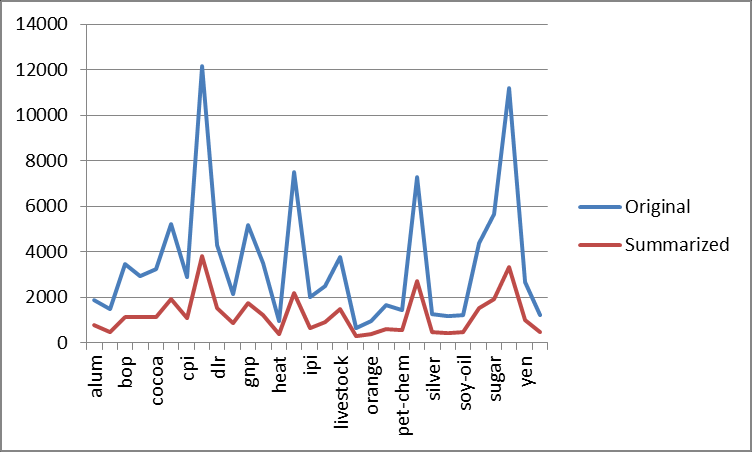
\includegraphics[width=0.9\columnwidth]{figures/DocumentClassificationAzadehDorna-000}
  \caption{Feature dimensionality reduction. }~\label{figureDimensionalityReduction}
\end{figure}

For comparative evaluation, the classification was performed and measured for both the original full-length documents and the summarized documents. 
The maximum and minimum number of documents for the training set was 388 and 7 respectively. 
As it is shown in figures~\ref{figurePrecision} and~\ref{figureRecall}, the precision and recall for different categories have improved noticeably using our approach. 
\begin{figure}
\centering
  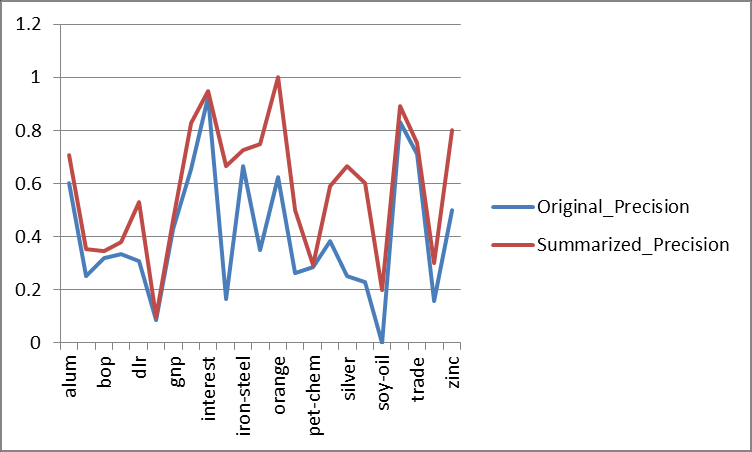
\includegraphics[width=0.9\columnwidth]{figures/DocumentClassificationAzadehDorna-002}
  \caption{Precision achieved for the original and the summarized feature set. }~\label{figurePrecision}
\end{figure}
\begin{figure}
\centering
  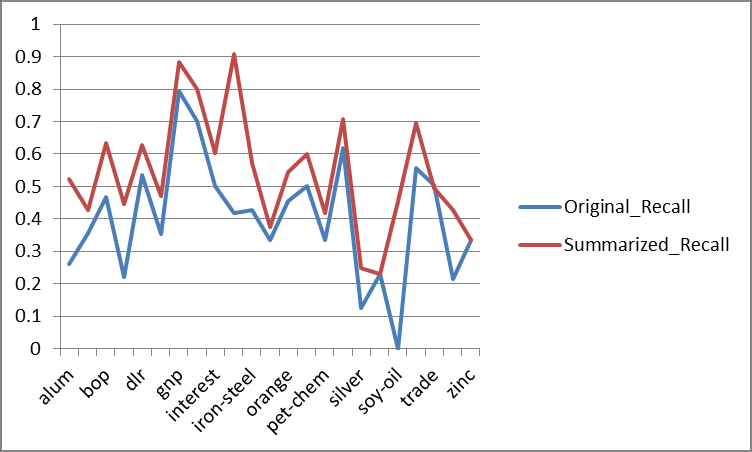
\includegraphics[width=0.9\columnwidth]{figures/DocumentClassificationAzadehDorna-004}
  \caption{Recall achieved for the original and the summarized feature set.}~\label{figureRecall}
\end{figure}
The classification performance determined by the F1-measure shown in figure~\ref{figureF1} indicates the positive impact of the summarization.
\begin{figure}
\centering
  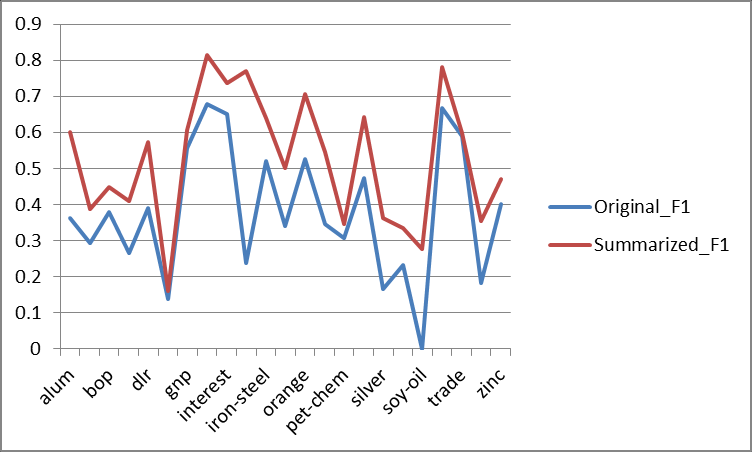
\includegraphics[width=0.9\columnwidth]{figures/DocumentClassificationAzadehDorna-006}
  \caption{F1-measure achieved for the original and the summarized feature set.}~\label{figureF1}
\end{figure}
The F1-mesure has increased significantly for the summarized documents in comparison with the full length documents.

The length of documents and the number of documents in the training set significantly influences the results. 
When at least one of these increases, the feature set will also increase in size. 
As a result of this, the possibility of co-occurrence of common words between categories increases and finally leads to the reduced Precision. 
A relatively large feature set may impact the Recall positively, but it affects the Precision negatively.
\textbf{No link and explanation for figure~\ref{figureSummary}}
\begin{figure}
\centering
  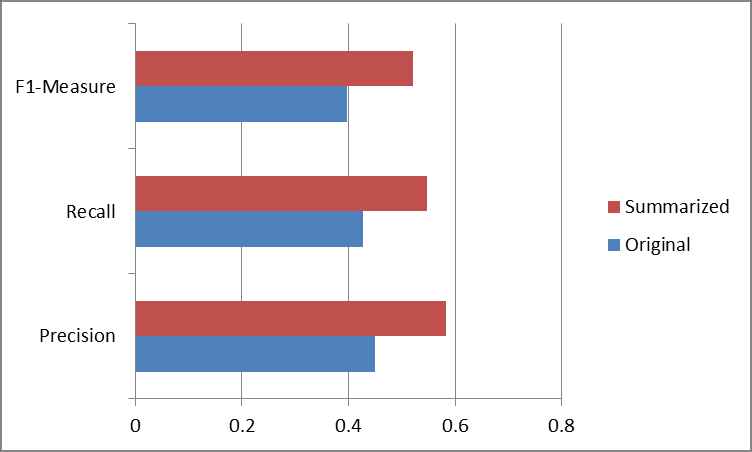
\includegraphics[width=0.9\columnwidth]{figures/DocumentClassificationAzadehDorna-008}
  \caption{F1-measure achieved for the original and the summarized feature set.}~\label{figureSummary}
\end{figure}

\section{Conclusion}\label{sectionConclusion}
\textbf{TODO: add link ot app recommendation}
The proposed document classification system utilizes the advantages of using
\textbf{...What? Sth is missing}
In this paper, we investigated the applying of a graph-based summarization approach to the document classification. 
The evaluation was performed for the original and summarized documents. 
First, we used the extractive summarization algorithm to reduce the number of features and solved the curse of dimension. 
Second, we showed how the extractive summarization could be effectively and usefully applied in KNN-classification for documents and improved the acquired results.


% Balancing columns in a ref list is a bit of a pain because you
% either use a hack like flushend or balance, or manually insert
% a column break.  http://www.tex.ac.uk/cgi-bin/texfaq2html?label=balance
% multicols doesn't work because we're already in two-column mode,
% and flushend isn't awesome, so I choose balance.  See this
% for more info: http://cs.brown.edu/system/software/latex/doc/balance.pdf
%
% Note that in a perfect world balance wants to be in the first
% column of the last page.
%
% If balance doesn't work for you, you can remove that and
% hard-code a column break into the bbl file right before you
% submit:
%
% http://stackoverflow.com/questions/2149854/how-to-manually-equalize-columns-
% in-an-ieee-paper-if-using-bibtex
%
% Or, just remove \balance and give up on balancing the last page.
%
\balance{}


% REFERENCES FORMAT
% References must be the same font size as other body text.
\bibliographystyle{SIGCHI-Reference-Format}
\bibliography{documentClassification}

\end{document}

%%% Local Variables:
%%% mode: latex
%%% TeX-master: t
%%% End:
